\section{Objective}
\begin{itemize}
	\item To examine the Superposition Theorem in multi-source linear DC networks.
	\item To experimentally prove that total branch currents equal the algebraic sum of responses from individual independent sources.
	\item To investigate the Maximum Power Transfer Theorem by observing load power variations across variable resistances.
	\item To trace the power-resistance profile experimentally and compare peak power conditions with theoretical predictions.
\end{itemize}

\section{Introduction}
This laboratory study evaluates two fundamental principles governing linear DC networks. The \textbf{Superposition Theorem} simplifies multi-source network analysis by calculating the isolated contribution of each independent source while deactivating others. The \textbf{Maximum Power Transfer Theorem} identifies the specific load condition that extracts peak power from a linear network. Both principles provide indispensable tools for network reduction and power optimization in resistive circuits.

\section{Theory}

\subsection{Part A: Superposition Theorem}

\subsubsection{Statement of the Theorem}
\begin{quote}
	\textit{In any linear, bilateral DC network containing multiple independent sources, the response in any branch equals the algebraic sum of the individual responses produced by each source acting independently while all other independent sources are deactivated.}
\end{quote}

\subsubsection{Deactivation of Independent Sources}
\begin{itemize}
	\item \textbf{Ideal Voltage Sources} are set to zero by replacing them with a \textbf{short circuit}.
	\item \textbf{Ideal Current Sources} are set to zero by replacing them with an \textbf{open circuit}.
\end{itemize}

\subsubsection{Mathematical Formulation}
For a branch current $I$ driven by sources $V_1$ and $V_2$:
\[
I = I' + I''
\]
where $I'$ is the branch current with $V_1$ active ($V_2$ shorted), and $I''$ is the branch current with $V_2$ active ($V_1$ shorted).

\subsubsection{Non-Applicability to Power Calculations}
Because electrical power follows a non-linear relationship ($P = I^2 R$), superposition cannot be applied directly to power:
\[
P_{\text{total}} \neq P_1 + P_2.
\]
Total current or voltage must be determined prior to calculating network power.

\subsection{Part B: Maximum Power Transfer Theorem}

\subsubsection{Statement of the Theorem}
A linear DC source network transfers maximum power to an external load $R_L$ when the load resistance matches the internal Thevenin resistance $R_{th}$ of the network:
\[
R_L = R_{th}.
\]

\subsubsection{Derivation}
For a network represented by $V_{th}$ and $R_{th}$ driving $R_L$:
\[
I_L = \frac{V_{th}}{R_{th}+R_L}, \qquad P_L = I_L^2 R_L = \frac{V_{th}^2 R_L}{(R_{th}+R_L)^2}.
\]
Setting $\dfrac{dP_L}{dR_L}=0$ yields $R_L = R_{th}$, resulting in:
\[
I_{L(\max)} = \frac{V_{th}}{2R_{th}}, \qquad P_{L(\max)} = \frac{V_{th}^2}{4R_{th}}.
\]
Under maximum power transfer, exactly $50\%$ of the total power is dissipated within the internal source resistance $R_{th}$.

\section{Apparatus and Components}
\begin{table}[h!]
	\centering
	\caption{List of Equipment and Components Used}
	\vspace{2mm}
	\begin{tabular}{llc}
		\toprule
		\rowcolor{blue!10}
		\textbf{Item Description} & \textbf{Specification / Rating} & \textbf{Quantity} \\
		\midrule
		\multicolumn{3}{l}{\textit{Part A: Superposition Theorem}} \\
		Dual-Channel DC Power Supply & RPS1, RPS2 (\qty{0}{\volt}--\qty{30}{\volt}) & 1 \\
		Resistor $R_1$ & \qty{325}{\ohm} & 1 \\
		Resistor $R_2$ & \qty{550}{\ohm} & 1 \\
		Resistor $R_3$ & \qty{960}{\ohm} & 1 \\
		\midrule
		\rowcolor{blue!10}
		\multicolumn{3}{l}{\textit{Part B: Maximum Power Transfer Theorem}} \\
		DC Power Supply ($V_{th}$) & \qty{8}{\volt} & 1 \\
		Series Resistor $R_i$ ($=R_{th}$) & \qty{663}{\ohm} & 1 \\
		Decade Resistance Box ($R_L$) & \qty{0}{\ohm}--\qty{5}{\kilo\ohm} & 1 \\
		\midrule
		\rowcolor{blue!10}
		\multicolumn{3}{l}{\textit{Common}} \\
		Digital Multimeter (DMM) & DC Voltage / Current & 1 \\
		Solderless Breadboard & Standard Tie-Point & 1 \\
		Connecting Wires & Jumper Wires & As required \\
		\bottomrule
	\end{tabular}
	\label{tab:apparatus5}
\end{table}

\section{Circuit Diagrams}

\subsection{Part A: Superposition Theorem}

\begin{figure}[h!]
	\centering
	\begin{circuitikz}[american, scale=1.0]
		\draw (0,0) to[V, l=$V_1$, invert] (0,3)
		(0,3) to[R, l=$R_1\,(\qty{325}{\ohm})$, i=$I_{R_1}$] (4,3)
		to[R, l=$R_2\,(\qty{550}{\ohm})$, i=$I_{R_2}$] (8,3)
		to[V, l=$V_2$] (8,0) -- (0,0);
		\draw (4,3) to[R, l=$R_3\,(\qty{960}{\ohm})$, i=$I_{R_3}$] (4,0);
		\draw (4,0) node[ground]{};
		\node at (4,3.3) [above right] {$V_A$};
	\end{circuitikz}
	\caption{Complete DC network driven simultaneously by voltage sources $V_1$ and $V_2$.}
	\label{fig:supcircuit1}
\end{figure}

\begin{figure}[h!]
	\centering
	\begin{circuitikz}[american, scale=1.0]
		\draw (0,0) to[V, l=$V_1$, invert] (0,3)
		(0,3) to[R, l=$R_1$, i=$I_{R_1}'$] (4,3)
		to[R, l=$R_2$, i=$I_{R_2}'$] (8,3) -- (8,0) -- (0,0);
		\draw (4,3) to[R, l=$R_3$, i=$I_{R_3}'$] (4,0);
		\draw (4,0) node[ground]{};
		\node at (8,1.5) [right] {\textbf{Short Circuit}};
	\end{circuitikz}
	\caption{Network response with $V_1$ active and $V_2$ short-circuited.}
	\label{fig:supcircuit2}
\end{figure}

\begin{figure}[h!]
	\centering
	\begin{circuitikz}[american, scale=1.0]
		\draw (0,0) -- (0,3)
		(0,3) to[R, l=$R_1$, i=$I_{R_1}''$] (4,3)
		to[R, l=$R_2$, i=$I_{R_2}''$] (8,3)
		to[V, l=$V_2$] (8,0) -- (0,0);
		\draw (4,3) to[R, l=$R_3$, i=$I_{R_3}''$] (4,0);
		\draw (4,0) node[ground]{};
		\node at (0,1.5) [left] {\textbf{Short Circuit}};
	\end{circuitikz}
	\caption{Network response with $V_2$ active and $V_1$ short-circuited.}
	\label{fig:supcircuit3}
\end{figure}

\subsection{Part B: Maximum Power Transfer Theorem}

\begin{figure}[h!]
	\centering
	\begin{circuitikz}[american, scale=1.0]
		\draw (0,0) to[battery1, l=$V_{th}$, invert] (0,3)
		(0,3) to[R, l=$R_i$] (4,3)
		to[R, l=$R_L$, i=$I_L$] (4,0) -- (0,0);
		\draw (4,0) node[ground]{};
	\end{circuitikz}
	\caption{Test circuit for maximum power transfer using $V_{th}=\qty{8}{\volt}$ and $R_i=\qty{663}{\ohm}$.}
	\label{fig:maxpowercircuit}
\end{figure}

\section{Experimental Procedure}

\subsection*{Part A: Verification of Superposition Theorem}
\begin{enumerate}
	\item Construct the circuit shown in Figure~\ref{fig:supcircuit1} using assigned resistor values ($R_1=\qty{325}{\ohm}$, $R_2=\qty{550}{\ohm}$, $R_3=\qty{960}{\ohm}$).
	\item Power both sources ($V_1$ and $V_2$) and record the combined current $I_{R_3}$.
	\item Deactivate $V_2$ using a short circuit (Figure~\ref{fig:supcircuit2}) and measure contribution $I_{R_3}'$.
	\item Restore $V_2$, short-circuit $V_1$ (Figure~\ref{fig:supcircuit3}), and measure contribution $I_{R_3}''$.
	\item Confirm that $I_{R_3} = I_{R_3}' + I_{R_3}''$ and repeat for the second voltage combination.
\end{enumerate}

\subsection*{Part B: Verification of Maximum Power Transfer Theorem}
\begin{enumerate}
	\item Assemble the equivalent network (Figure~\ref{fig:maxpowercircuit}) with $V_{th}=\qty{8}{\volt}$ and $R_i=\qty{663}{\ohm}$.
	\item Connect the decade resistance box as variable load $R_L$.
	\item Adjust $R_L$ across values ranging below and above $R_i$.
	\item Measure $I_L$ at each step and evaluate load power $P_L$.
	\item Plot $P_L$ versus $R_L$ to locate the resistance corresponding to maximum power delivery.
\end{enumerate}

\section{Theoretical Calculations}

\subsection{Part A: Superposition Theorem}
Using fixed resistances $R_1=\qty{325}{\ohm}$, $R_2=\qty{550}{\ohm}$, $R_3=\qty{960}{\ohm}$:

\subsubsection*{Case 1: Only $V_1$ Active ($V_2$ Short-Circuited)}
\[
R_{23} = \frac{R_2 R_3}{R_2+R_3} = \qty{349.67}{\ohm}, \qquad
R_{\text{eq1}} = R_1+R_{23} = \qty{674.67}{\ohm}.
\]
\[
I_{\text{total}}' = \frac{V_1}{R_{\text{eq1}}}, \qquad V_A' = I_{\text{total}}' \times R_{23}, \qquad I_{R_3}' = \frac{V_A'}{R_3}.
\]

\subsubsection*{Case 2: Only $V_2$ Active ($V_1$ Short-Circuited)}
\[
R_{13} = \frac{R_1 R_3}{R_1+R_3} = \qty{242.80}{\ohm}, \qquad
R_{\text{eq2}} = R_2+R_{13} = \qty{792.80}{\ohm}.
\]
\[
I_{\text{total}}'' = \frac{V_2}{R_{\text{eq2}}}, \qquad V_A'' = I_{\text{total}}'' \times R_{13}, \qquad I_{R_3}'' = \frac{V_A''}{R_3}.
\]

\subsubsection*{Trial 1 ($V_1=\qty{10}{\volt}$, $V_2=\qty{10}{\volt}$)}
\[
I_{R_3}' = \qty{5.39}{\milli\ampere}, \qquad I_{R_3}'' = \qty{3.19}{\milli\ampere}, \qquad I_{R_3} = \qty{8.58}{\milli\ampere} \approx \qty{8.59}{\milli\ampere}.
\]

\subsubsection*{Trial 2 ($V_1=\qty{15}{\volt}$, $V_2=\qty{10}{\volt}$)}
\[
I_{R_3}' = \qty{8.09}{\milli\ampere}, \qquad I_{R_3}'' = \qty{3.19}{\milli\ampere}, \qquad I_{R_3} = \qty{11.28}{\milli\ampere} \approx \qty{11.29}{\milli\ampere}.
\]

\subsection{Part B: Maximum Power Transfer Theorem}
For $V_{th}=\qty{8}{\volt}$ and $R_i=\qty{663}{\ohm}$:
\[
I_L = \frac{V_{th}}{R_{th}+R_L}, \qquad P_L = I_L^2 R_L.
\]
Peak power occurs at $R_L = R_{th} = \qty{663}{\ohm}$:
\[
P_{L(\max)} = \frac{V_{th}^2}{4R_{th}} = \qty{24.13}{\milli\watt} \approx \qty{24.12}{\milli\watt}.
\]

\section{Data Collection}

\subsection{Part A: Superposition Theorem}

\begin{table}[h!]
	\centering
	\caption{Superposition Verification -- Trial 1 ($V_1=\qty{10}{\volt}$, $V_2=\qty{10}{\volt}$)}
	\vspace{2mm}
	\begin{tabular}{lcccc}
		\toprule
		\rowcolor{blue!10}
		\textbf{Configuration} & \textbf{$V_1$ (V)} & \textbf{$V_2$ (V)} & \textbf{Measured $I_{R_3}$ (mA)} & \textbf{Calculated $I_{R_3}$ (mA)} \\
		\midrule
		Both Sources Active & 10 & 10 & 8.61 & 8.59 \\
		Only $V_1$ Active & 10 & 0 & 5.36 & 5.39 \\
		Only $V_2$ Active & 0 & 10 & 3.21 & 3.19 \\
		\bottomrule
	\end{tabular}
	\label{tab:supdata1}
\end{table}

\begin{table}[h!]
	\centering
	\caption{Superposition Verification -- Trial 2 ($V_1=\qty{15}{\volt}$, $V_2=\qty{10}{\volt}$)}
	\vspace{2mm}
	\begin{tabular}{lcccc}
		\toprule
		\rowcolor{blue!10}
		\textbf{Configuration} & \textbf{$V_1$ (V)} & \textbf{$V_2$ (V)} & \textbf{Measured $I_{R_3}$ (mA)} & \textbf{Calculated $I_{R_3}$ (mA)} \\
		\midrule
		Both Sources Active & 15 & 10 & 11.3 & 11.29 \\
		Only $V_1$ Active & 15 & 0 & 8.11 & 8.09 \\
		Only $V_2$ Active & 0 & 10 & 3.2 & 3.19 \\
		\bottomrule
	\end{tabular}
	\label{tab:supdata2}
\end{table}

\subsection{Part B: Maximum Power Transfer Theorem}

\begin{table}[h!]
	\centering
	\caption{Power Transfer Measurement Log ($V_{th}=\qty{8}{\volt}$, $R_i=\qty{663}{\ohm}$)}
	\vspace{2mm}
	\resizebox{\textwidth}{!}{%
		\begin{tabular}{cccccc}
			\toprule
			\rowcolor{blue!10}
			\textbf{S.No.} & \textbf{$R_L$ ($\Omega$)} & \textbf{Measured $I_L$ (mA)} & \textbf{Calculated $I_L$ (mA)} & \textbf{Observed $P_L$ (mW)} & \textbf{Calculated $P_L$ (mW)} \\
			\midrule
			1 & 99.6  & 10.70 & 10.50 & 11.30 & 10.92 \\
			2 & 327   & 8.22  & 8.08  & 22.10 & 21.80 \\
			3 & 460   & 7.23  & 7.12  & 24.00 & 23.30 \\
			4 & \textbf{663 (Peak)} & \textbf{6.14} & \textbf{6.03} & \textbf{24.90} & \textbf{24.12} \\
			5 & 973   & 4.97  & 4.89  & 23.90 & 23.20 \\
			6 & 2152  & 2.88  & 2.84  & 17.80 & 17.30 \\
			7 & 3232  & 2.07  & 2.05  & 13.90 & 13.60 \\
			\bottomrule
		\end{tabular}%
	}
	\label{tab:maxpowerdata}
\end{table}

\begin{figure}[h!]
	\centering
	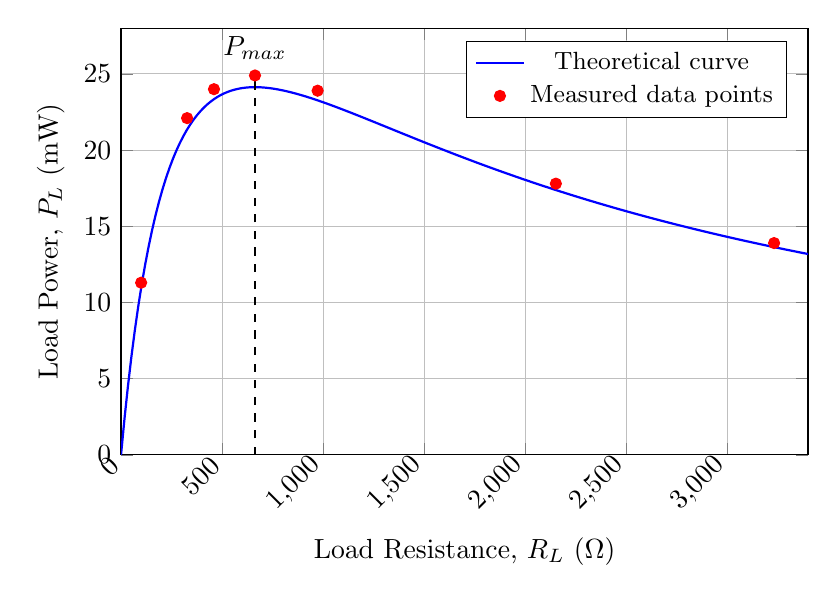
\begin{tikzpicture}
		\begin{axis}[
			width=0.85\textwidth,
			height=7cm,
			xlabel={Load Resistance, $R_L$ ($\Omega$)},
			ylabel={Load Power, $P_L$ (mW)},
			xmin=0, xmax=3400,
			ymin=0, ymax=28,
			grid=major,
			legend pos=north east,
			legend style={font=\small},
			x tick label style={rotate=45, anchor=east}, 
			]
			\addplot[domain=0:3400, samples=200, thick, blue] {64000*x/(663+x)^2};
			\addlegendentry{Theoretical curve}
			\addplot[only marks, mark=*, red, mark size=2pt] coordinates {
				(99.6,11.30) (327,22.10) (460,24.00) (663,24.90) (973,23.90) (2152,17.80) (3232,13.90)
			};
			\addlegendentry{Measured data points}
			\draw[dashed] (axis cs:663,0) -- (axis cs:663,24.90);
			\node[above] at (axis cs:663,25.3) {$P_{max}$};
		\end{axis}
	\end{tikzpicture}
	\caption{Load power $P_L$ versus load resistance $R_L$, illustrating peak delivery at $R_L = R_i = \qty{663}{\ohm}$.}
	\label{fig:maxpowergraph}
\end{figure}

\section{Result Analysis}

\subsection{Part A: Superposition Theorem}
The algebraic summation of individual current responses closely matches the multi-source total:
\begin{itemize}
	\item \textbf{Trial 1}: $I_{R_3}' + I_{R_3}'' = \qty{5.36}{\milli\ampere} + \qty{3.21}{\milli\ampere} = \qty{8.57}{\milli\ampere}$ (Measured combined = \qty{8.61}{\milli\ampere}, percentage error $= 0.23\%$).
	\item \textbf{Trial 2}: $I_{R_3}' + I_{R_3}'' = \qty{8.11}{\milli\ampere} + \qty{3.2}{\milli\ampere} = \qty{11.31}{\milli\ampere}$ (Measured combined = \qty{11.3}{\milli\ampere}, percentage error $= 0.09\%$).
\end{itemize}

\subsection{Part B: Maximum Power Transfer Theorem}
Peak load power ($P_L=\qty{24.90}{\milli\watt}$) was recorded at $R_L=\qty{663}{\ohm}$, matching internal series resistance $R_i=\qty{663}{\ohm}$. The deviation between observed and calculated maximum power is $3.23\%$.

\section{Discussion and Sources of Error}
Experimental deviations remained under $3.5\%$, influenced by:
\begin{enumerate}
	\item \textbf{Resistor Tolerances:} Discrepancies between nominal and real component values.
	\item \textbf{Supply Regulation:} Minor fluctuations in supply output voltage under varying branch currents.
	\item \textbf{Instrument Loading:} Non-ideal internal resistance of measurement devices.
	\item \textbf{Decade Box Resolution:} Small contact and lead resistances within the variable resistance box.
\end{enumerate}

\section{Conclusion}
Both network theorems were confirmed experimentally within minimal error bounds. Superposition held true for linear currents across independent source configurations. Furthermore, maximum power delivery occurred precisely when load resistance equaled source impedance.

\section{References}
\begin{tcolorbox}[colback=gray!5, colframe=gray!40, arc=2mm]
	\begin{enumerate}
		\item Alexander, C. K., \& Sadiku, M. N. O. (2016). \textit{Fundamentals of Electric Circuits} (6th ed.). McGraw-Hill Education.
		\item Hayt, W. H., Kemmerly, J. E., \& Durbin, S. M. (2012). \textit{Engineering Circuit Analysis} (8th ed.). McGraw-Hill Education.
		\item Boylestad, R. L. (2015). \textit{Introductory Circuit Analysis} (13th ed.). Pearson.
	\end{enumerate}
\end{tcolorbox}